\documentclass[12pt,compress,aspectratio=169]{beamer}
\usetheme{metropolis}
\setbeamersize{text margin left=.5cm,text margin right=.5cm}
\usepackage[lf]{carlito}
\usepackage{siunitx}
\usepackage{tikz}
\usepackage{mathpazo}
\usepackage{bm}
\usepackage{mathtools}
\usepackage[ISO]{diffcoeff}
\diffdef{}{ op-symbol=\mathsf{d} }
\usepackage{xcolor,colortbl}

\setmonofont{Ubuntu Mono}
\setlength{\parskip}{0pt}
\renewcommand{\baselinestretch}{1}

\sisetup{
  inter-unit-product=\cdot,
  per-mode=symbol
}

\tikzset{
  >=latex
}

%\newcommand{\iii}{\hat{\bm\imath}}
%\newcommand{\jjj}{\hat{\bm\jmath}}
%\newcommand{\kkk}{\hat{\bm k}}

\usepackage{pgfplots}

\usetikzlibrary{decorations.pathmorphing,patterns}

\title{Class 10: Harmonic Motion}
\subtitle{Advanced Placement Physics C}
\author[TML]{Dr.\ Timothy Leung}
\institute{Olympiads School}
\date{Updated: Summer 2022}

\newcommand{\pic}[2]{
  \includegraphics[width=#1\textwidth]{#2}
}
\newcommand{\eq}[2]{
  \vspace{#1}{\Large
    \begin{displaymath}
      #2
    \end{displaymath}
  }
}
%\newcommand{\iii}{\ensuremath\hat{\bm{\imath}}}
%\newcommand{\jjj}{\ensuremath\hat{\bm{\jmath}}}
%\newcommand{\kkk}{\ensuremath\hat{\bm{k}}}
\newcommand{\iii}{\ensuremath\hat\imath}
\newcommand{\jjj}{\ensuremath\hat\jmath}
\newcommand{\kkk}{\ensuremath\hat k}



\begin{document}

\begin{frame}
  \maketitle
\end{frame}


\section{Hooke's Law}

\begin{frame}{Hooke's Law}
  Hooke's law for an ideal spring relates the \textbf{spring force} $\vec F_e$
  exerted by a compressed or stretched spring onto another object to the
  \textbf{spring constant} $k$ (the stiffness of the spring, also called
  \emph{Hooke's constant}, \emph{force constant}, or the \emph{spring rate}) of
  the spring, and the spring's displacement $\vec x$:

  \eq{-.1in}{
    \boxed{\vec F_s=-k\vec x}
  }
  \begin{center}
    \begin{tabular}{l|c|c}
      \rowcolor{pink}
      \textbf{Quantity} & \textbf{Symbol} & \textbf{SI Unit} \\ \hline
      Spring force                    & $\vec F_e$ & \si\newton \\
      Spring constant                 & $k$        & \si{\newton\per\metre}\\
      Amount of extension/compression & $\vec x$   & \si\metre
    \end{tabular}
  \end{center}
\end{frame}



\begin{frame}{Elastic Potential Energy}
  Applying Hooke's law in the work equation gives the amount of \textbf{elastic
    potential energy} stored in the spring when it is compressed or stretched:

  \eq{-.1in}{
    W=\int^{x_2}_{x_1}\vec F_s\cdot\dl\vec x=-\int^{x_2}_{x_1}kx\dl x
    =-\frac12kx^2\Big|^{x_2}_{x_1}=-\Delta U_e
  }

  where elastic potential energy is defined as

  \eq{-.1in}{
    \boxed{U_e=\frac12kx^2}
  }
\end{frame}



\section{Spring-Mass}

\begin{frame}{Horizontal Spring-Mass System}
  Consider the forces acting on a mass connected horizontally to a spring
  without friction
  \begin{center}
    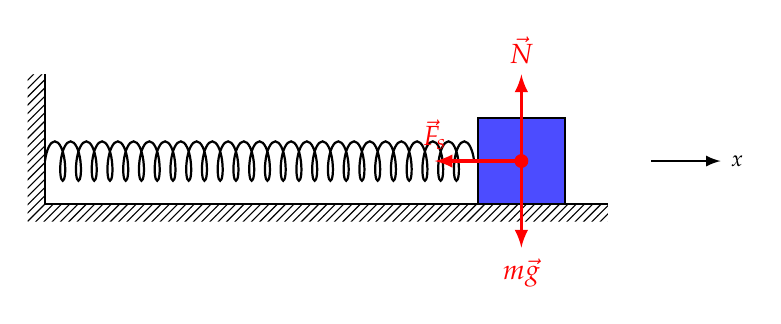
\begin{tikzpicture}[scale=1.1]
      \draw[thick,fill=blue!70] (5,.5) rectangle (6,1.5);
      \draw[thick,
        decoration={aspect=.3,segment length=2mm, amplitude=2.5mm, coil},
        decorate] (0,1)--(5,1);
      \fill[pattern=north east lines] (6.5,.5)--(6.5,.3)--(-0.2,.3)
      --(-.2,2)--(0,2)--(0,.5)--cycle;
      \draw[thick] (6.5,.5)--(0,.5)--(0,2);
      \draw[->,thick](7,1)--(7.8,1) node[right]{\footnotesize $x$};
      
      \fill[red] (5.5,1) circle(.08);
      \begin{scope}[very thick,->,red]
        \draw (5.5,1)--(5.5,0) node[below]{$m\vec g$};
        \draw (5.5,1)--(5.5,2) node[above]{$\vec N$};
        \draw (5.5,1)--(4.5,1) node[above]{$\vec F_s$};
      \end{scope}
    \end{tikzpicture}
  \end{center}
  $m\vec g$ and $\vec N$ cancel out, so net force is due only to spring force
  $\vec F_s=-k\vec x$ along the $x$-axis. This is true both when the spring is
  in compression or extension. (The spring is in extension in the diagram.)
\end{frame}



\begin{frame}{Horizontal Spring-Mass System}
  Applying second law of motion in the $x$-direction:

  \eq{-.1in}{
    \sum F=F_s=ma\quad\longrightarrow\quad-kx=m\ddot x
  }

  This is a
  \emph{second-order ordinary differential equation with constant
    coefficients}. In standard form:

  \eq{-.1in}{
    \ddot x+\frac kmx=0
  }
  

\end{frame}



\begin{frame}{Mass on a Spring}

  The solution to the equation is a function $x(t)$ where the second time
  derivative $\ddot x$ looks like $x$ but with a negative sign

  \eq{-.1in}{
    \ddot x+\frac kmx=0
  }

  The obvious choices are the trigonometric functions $\sin(t)$ and $\cos(t)$.
  Starting with this general form:
    
  \eq{-.1in}{
    x(t)=A\cos(\omega_0 t-\phi)
  }
  
  Cosine is usually preferred over sine because $\cos(0)=1$, consistent with
  the fact that oscillations usually begin at maximum amplitude $A$ at $t=0$,
  and therefore $\phi=0$. Mathematically, the two functions only differ in
  $\phi$
\end{frame}



\begin{frame}{Mass on a Spring}

  \eq{0in}{
    \boxed{\ddot x+\frac kmx=0}
  }
  
  Starting with the general form and take the time derivatives to obtain the
  velocity and acceleration of the mass:
 
  \vspace{-.2in}{\large
    \begin{align*}
      x(t)&=A\cos(\omega_0 t-\phi)\\
      v(t)&=-A\omega_0\sin(\omega_0 t-\phi)\\
      a(t)&=-A\omega_0^2\cos(\omega_0 t-\phi)=-\omega_0^2x
    \end{align*}
  }
  
  where $\omega_0$ is the angular frequency of the oscillation, $A$ is the
  amplitude, and $\phi$ is the phase shift
\end{frame}



\begin{frame}{Mass on a Spring: Angular Frequency}
  Substituting expressions of $x(t)$ and $a(t)=\ddot x$ back into the ODE, we
  find that the solution is satisfied if $\omega_0$ is related to the spring
  constant and mass by:

  \eq{-.1in}{
    \boxed{
      \omega_0=\sqrt{\frac km}
    }  }

  The angular frequency for the (undamped) simple harmonic oscillator is called
  the \textbf{natural frequency}. The period ($T_0$) and frequency ($f_0$) of
  the undamped harmonic oscillator are then given by:

  \eq{-.1in}{
    f_0=\frac{\omega_0}{2\pi}=\frac1{2\pi}\sqrt{\frac km}\quad\quad
    T_0=\frac1{f_0}=2\pi\sqrt{\frac mk}
  }
  
  Angular frequency, frequency, and period do not depend on amplitude $A$
\end{frame}



\begin{frame}{Displacement, Velocity and Acceleration}
  \begin{columns}
    \column{.4\textwidth}

    \begin{align*}
      x(t)&=A\cos(\omega_0 t-\phi)\\
      v(t)&=-A\omega_0\sin(\omega_0 t-\phi)\\
      a(t)&=-A\omega_0^2\cos(\omega_0 t-\phi)=-\omega_0^2x
    \end{align*}

    \column{.6\textwidth}
    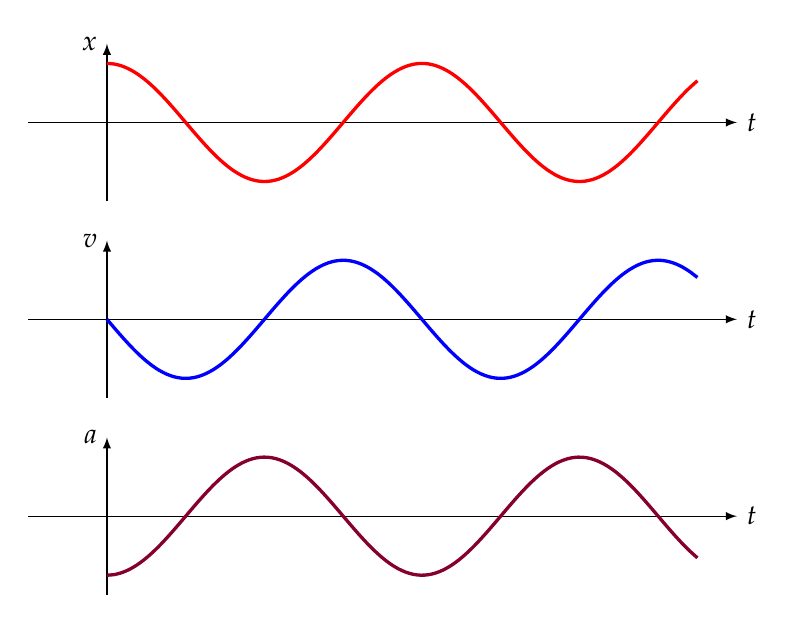
\begin{tikzpicture}[yscale=.5]
      \draw[->](0,-2)--(0,2)  node[left]{$x$};
      \draw[->](-1,0)--(8,0) node[right]{$t$};
      \draw[red,very thick,smooth,samples=80,domain=0:7.5]
      plot(\x,{1.5*cos(90*\x)});
      
      \draw[->](0,-7)--(0,-3)  node[left]{$v$};
      \draw[->](-1,-5)--(8,-5) node[right]{$t$};
      \draw[blue,very thick,smooth,samples=80,domain=0:7.5]
      plot(\x,{-1.5*sin(90*\x)-5});
      
      \draw[->](0,-12)--(0,-8)  node[left]{$a$};
      \draw[->](-1,-10)--(8,-10) node[right]{$t$};
      \draw[purple!70!black,very thick,smooth,samples=80,domain=0:7.5]
      plot(\x,{-1.5*cos(90*\x)-10});
    \end{tikzpicture}
  \end{columns}
\end{frame}



\begin{frame}{Side Note \#1}
  \textbf{Side Note \#1:} For anyone who has more experiences with calculus,
  you will know that the solution to any ODE is the linear combination of
  \emph{all} possible solutions, i.e.:

  \eq{-.1in}{
    x(t)=c_1\sin(\omega t)+c_2\cos(\omega t)
  }

  Where $c_1$ and $c_2$ are constant coefficients based on the initial
  conditions (position and velocity). Trigonometric identities can be used to
  show that the solution form shown in previous slides is identical.
\end{frame}



\begin{frame}{Side Note \#2}
  \textbf{Side Note \#2:} Another function that can be tried as a solution to
  the ODE is the exponential function, where its derivatives is related to the
  function itself. However, the second derivative of $e^{\omega t}$ does not have
  the negative sign that is needed to solve the problem.

  \eq{-.1in}{
    x(t)=e^{\omega t}\quad\rightarrow\quad
    \ddot x=\omega^2 e^{\omega t}=\omega^2x
  }

  But if the exponential function is \emph{imaginary}:

  \eq{-.1in}{
    x(t)=e^{i\omega t}
  }

  \vspace{-.1in}Then\ldots
\end{frame}



\begin{frame}{Side Note \#2}
  The second derivative \emph{does} in fact have the negative sign:

  \vspace{-.2in}{\large
    \begin{align*}
      x&=e^{i\omega t}\\
      \dot x&=i\omega e^{i\omega t}\\
      \ddot x&=i^2\omega^2 e^{i\omega t}=-\omega^2 e^{i\omega t}
    \end{align*}
  }
  
  \vspace{-.2in}This should not come as a surprise, since the complex
  exponential function and the sinusoidal functions are related:

  \eq{-.1in}{
    e^{i\omega t}=\cos(\omega t)+i\sin(\omega t)
  }
\end{frame}



\begin{frame}{Vertical Spring-Mass System}
  \begin{columns}
    \column{.17\textwidth}
    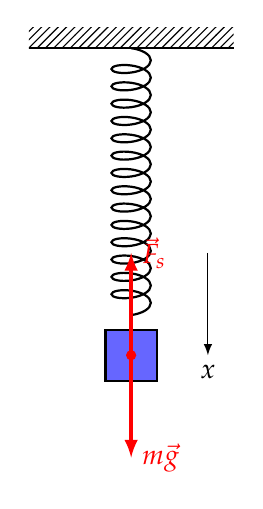
\begin{tikzpicture}[scale=1.3]
      \draw[thick,fill=blue!60] (.75,1.75) rectangle (1.25,2.25);
      \draw[thick,
        decoration={aspect=.4,segment length=2.2mm, amplitude=2.5mm, coil},
        decorate] (1,5)--(1,2.25); 
      \fill[pattern=north east lines] (0,5) rectangle (2,5.2);
      \draw[thick] (0,5)--(2,5);
      \draw[->](1.75,3)--(1.75,2) node[below]{$x$};
      \begin{scope}[very thick,->,red]
        \draw(1,2)--(1,1)node[right]{$m\vec g$};
        \draw(1,2)--(1,3)node[right]{$\vec F_s$};
      \end{scope}
      \fill[red](1,2) circle(.05);
    \end{tikzpicture}

    \column{.85\textwidth}
    For a vertical spring-mass system, we must consider the
    {\color{purple}weight} as well:

    \eq{-.1in}{
      {\color{purple}mg}-kx=m\ddot x%\frac{d^2x}{dt^2}
    }

    But since $mg$ is a constant, the only change is the addition of a constant
    $B$ in the expression of $x(t)$:
    
    \vspace{-.25in}{\large
      \begin{align*}
        x(t)&=A\cos(\omega_0 t-\phi) +B\\
        v(t)&=-A\omega_0\sin(\omega_0 t-\phi)\\
        a(t)&=-A\omega_0^2\cos(\omega_0 t-\phi)
      \end{align*}
    }
  \end{columns}
\end{frame}



\begin{frame}{Vertical Spring-Mass System}
  \begin{columns}
    \column{.17\textwidth}
    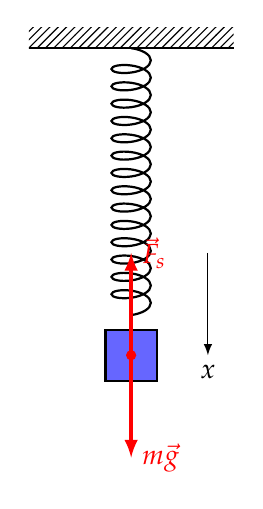
\begin{tikzpicture}[scale=1.3]
      \draw[thick,fill=blue!60] (.75,1.75) rectangle (1.25,2.25);
      \draw[thick,
        decoration={aspect=.4,segment length=2.2mm, amplitude=2.5mm, coil},
        decorate] (1,5)--(1,2.25); 
      \fill [pattern=north east lines] (0,5) rectangle (2,5.2);
      \draw[thick] (0,5)--(2,5);
      \draw[->](1.75,3)--(1.75,2) node[below]{$x$};
      \begin{scope}[very thick,->,red]
        \draw(1,2)--(1,1)node[right]{$m\vec g$};
        \draw(1,2)--(1,3)node[right]{$\vec F_s$};
      \end{scope}
      \fill[red](1,2) circle(.05);
    \end{tikzpicture}

    \column{.85\textwidth}
    $B$ is found by substituting $x$ and $\ddot x$ into the ODE.
    It is stretching of the spring due to its weight:
    
    \eq{-.1in}{
      B=\frac{mg}k
    }

    Angular frequency (natural frequency) remains the same as the horizontal
    case:

    \eq{-.1in}{
      \omega_0=\sqrt{\frac km}
    }
  \end{columns}
\end{frame}



\begin{frame}{Conservation of Energy in a Spring-Mass System}

  In the spring-mass systems, if there are no frictional losses, then the only
  forces doing work are the spring force (horizontal and vertical) and gravity
  (vertical). Both forces are \emph{conservative}, therefore the total
  mechanical energy is conserved:

  \eq{-.1in}{
    K_1 + U_{e1} + U_{g1} = K_2 + U_{e2} + U_{g2}
  }
  
  For the horizontal spring-mass system, the total energy of the simple harmonic
  oscillator is:
    
  \eq{-.1in}{
    \boxed{E_T=\frac12kA^2}
  }
\end{frame}



\begin{frame}{Simple Example}
  \textbf{Example 2:} A mass suspended from a spring is oscillating up and
  down. Consider the following two statements:
  \begin{enumerate}
  \item At some point during the oscillation, the mass has zero velocity but it
    is accelerating
  \item At some point during the oscillation, the mass has zero velocity and
    zero acceleration.
  \end{enumerate}

  \begin{enumerate}[(A)]
  \item Both occur at some time during the oscillation
  \item Neither occurs during the oscillation
  \item Only (1) occurs
  \item Only (2) occurs
  \end{enumerate}
\end{frame}



\begin{frame}{Another Example}
  \textbf{Example 3:} An object of mass \SI5{\kilo\gram} hangs from a spring
  and oscillates with a period of \SI{.5}\second. By how much will the
  equilibrium length of the spring be shortened when the object is removed.
  \begin{enumerate}[(A)]
  \item\SI{0.75}{\centi\metre}
  \item\SI{1.50}{\centi\metre}
  \item\SI{3.13}{\centi\metre}
  \item\SI{6.20}{\centi\metre}
  \end{enumerate}
\end{frame}



\section{Simple Pendulum}

\begin{frame}{What About a Simple Pendulum?}
  \begin{columns}
    \column{.75\textwidth}
    \begin{itemize}
    \item Pendulums also exhibit oscillatory motion
    \item In a \textbf{simple pendulum}, all of the mass is concentrated at the
      end point 
    \item There are two forces acting on the mass: weight $mg$ and tension $T$
    \item It has already been shown previously that when the mass is deflected
      by an angle $\phi$, the tangential force is $F_t=-mg\sin\phi$
    \item No need to worry about the radial direction; it does not have to do
      with the restoring force
    \end{itemize}

    \column{.25\textwidth}
    \centering 
    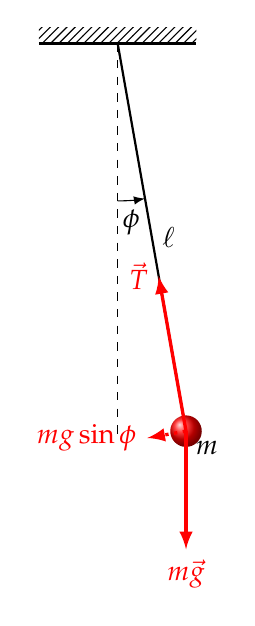
\begin{tikzpicture}
      \fill[pattern=north east lines] (-1,0) rectangle (1,0.2);
      \draw[thick](-1,0)--(1,0);
      \begin{scope}[rotate=10]
        \draw[thick](0,0)--(0,-5) node[midway,right]{$\ell$};
        \shade[ball color=red](0,-5) circle(.2) node[below right]{$m$};
        \begin{scope}[red,very thick,->]
          \draw[dotted](0,-5)--(-0.5,-5) node[left]{$mg\sin\phi$};
          \draw(0,-5)--(0,-3) node[left]{$\vec T$};
          \draw[rotate around={-10:(0,-5)}](0,-5)--(0,-6.5)
          node[below]{$m\vec g$};
        \end{scope}
      \end{scope}
      \draw[dashed,thin](0,0)--(0,-5);
      \draw[->](0,-2) arc(270:280:2) node[midway,below]{$\phi$};
    \end{tikzpicture}
  \end{columns}
\end{frame}



\begin{frame}{The Simple Pendulum}
  \begin{columns}
    \column{.75\textwidth}
    Substitute $F_t$ into second law of motion, and cancelling $m$:

    \eq{-.1in}{
      F_t=ma_t\quad\rightarrow\quad -g\sin\phi=\ell\ddot{\phi}
    }

    Solving this ODE in its present form is difficult because of the
    $\sin\phi$ term. However, the series expansion of the sine function:

    \eq{-.1in}{
      \sin\phi=\phi-\frac{\phi^3}{3!}+\frac{\phi^5}{5!}-\frac{\phi^7}{7!}+
      \cdots
    }
    
    shows that for small angles, $\sin\phi\approx\phi$
    
    \column{.25\textwidth}
    \centering
    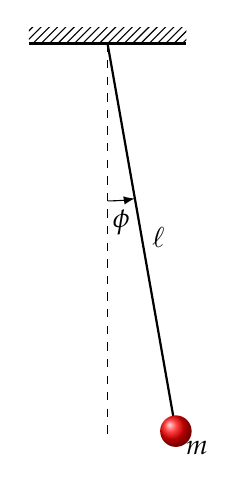
\begin{tikzpicture}
      \fill[pattern=north east lines] (-1,0) rectangle (1,0.2);
      \draw[thick](-1,0)--(1,0);
      \begin{scope}[rotate=10]
        \draw[thick](0,0)--(0,-5) node[midway,right]{$\ell$};
        \shade[ball color=red](0,-5) circle(.2) node[below right]{$m$};
      \end{scope}
      \draw[dashed,thin](0,0)--(0,-5);
      \draw[->](0,-2) arc(270:280:2) node[midway,below]{$\phi$};
    \end{tikzpicture}
  \end{columns}
\end{frame}



\begin{frame}{The Simple Pendulum}
  \begin{columns}
    \column{.75\textwidth}
    For small angles of $\phi$, the ODE reduces to the same form as the
    spring-mass system

    \eq{-.1in}{
      \ddot{\phi}+\frac g\ell\phi=0
    }

    So how small is ``small angle''? That depends on what tolerance (the
    number of significant figures) is needed in the answer.
    
    \column{.25\textwidth}
    \centering
    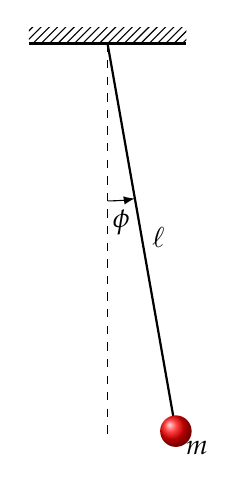
\begin{tikzpicture}
      \fill[pattern=north east lines] (-1,0) rectangle (1,0.2);
      \draw[thick](-1,0)--(1,0);
      \begin{scope}[rotate=10]
        \draw[thick](0,0)--(0,-5) node[midway,right]{$\ell$};
        \shade[ball color=red](0,-5) circle(.2) node[below right]{$m$};
      \end{scope}
      \draw[dashed,thin](0,0)--(0,-5);
      \draw[->](0,-2) arc(270:280:2) node[midway,below]{$\phi$};
    \end{tikzpicture}
  \end{columns}
\end{frame}



\begin{frame}{Ordinary Differential Equation for the Pendulum}
  The solution for $\phi(t)$ is a sinusoidal function, like the spring-mass
  system:

  \eq{-.1in}{
    \boxed{\phi(t)=\Phi\cos(\omega_0 t-\beta)}
  }

  where $\Phi$ is the maximum deflection (amplitude), and angular frequency
  (natural frequency) of the oscillation $\omega_0$ is given by:
    
  \eq{-.1in}{
    \boxed{
      \omega_0=\sqrt{\frac g\ell}
    }
  }

  and $\beta$ is a phase shift based on the initial condition of the pendulum.
  If the oscillation begins at amplitude, then $\beta=0$.
\end{frame}



\begin{frame}{How Good is the Small Angle Approximation?}
  \begin{center}
    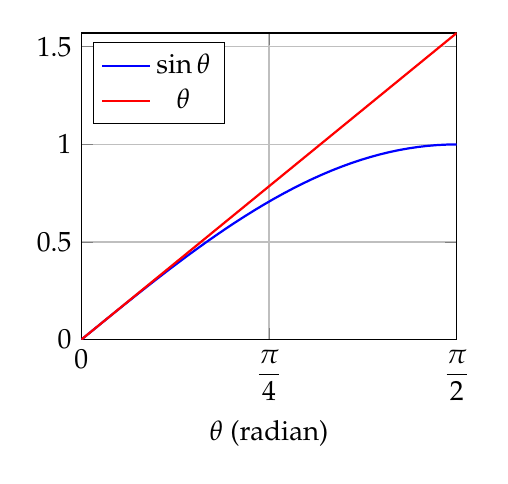
\begin{tikzpicture}
      \begin{axis}[
          width=2.5in,
          xmin=0,xmax=pi/2,
          ymin=0,ymax=pi/2,
          xlabel=$\theta$ (radian),
          xtick={0,pi/4,pi/2},
          xticklabels={0,$\dfrac\pi4$,$\dfrac\pi2$},
          grid = both,
          legend pos=north west,
        ]
        \addplot[
          color=blue,
          domain=0:pi/2,
          samples=40,
          style={thick}]{sin(x*180/pi)};
        \addlegendentry{$\sin\theta$};
        \addplot[
          color=red,
          domain=0:pi/2,
          samples=40,
          thick]{x};
        \addlegendentry{$\theta$};
      \end{axis}
    \end{tikzpicture}
    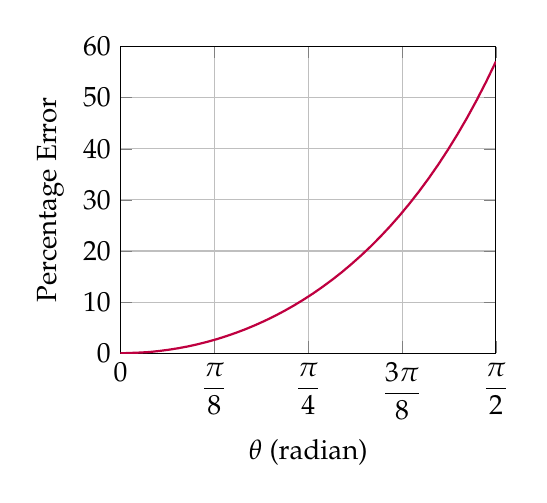
\begin{tikzpicture}
      \begin{axis}[
          width=2.5in,
          ylabel=Percentage Error,
          xmin=0,xmax=pi/2,
          ymin=0,ymax=60,
          xlabel=$\theta$ (radian),
          xtick={0,pi/8,pi/4,3*pi/8,pi/2},
          xticklabels={
            0,$\dfrac\pi8$,$\dfrac\pi4$,$\dfrac{3\pi}8$,$\dfrac\pi2$
          },
          ytick={0,10,...,60},
          legend pos=north west,
          grid = both,
        ]
        \addplot[
          color=purple,
          domain=0:pi/2,
          samples=40,
          style=thick
        ]{abs(sin(x*180/pi)-x)/sin(x*180/pi)*100};
      \end{axis}
    \end{tikzpicture}
  \end{center}
  What the maximum angle of deflection can be depends on the accuracy the answer
  requires.
\end{frame}



\begin{frame}{Pendulum Example Problem}
  \textbf{Example:} A simple pendulum consists of a mass $m$ attached to a
  light string of length $l$. If the system is oscillating through small
  angles, which of the following is true
  \begin{enumerate}[(A)]
  \item The frequency is independent of the acceleration due to gravity, $g$.
  \item The period depends on the amplitude of the oscillation.
  \item The period is independent of the mass $m$.
  \item The period is independent of the length $l$.
  \end{enumerate}
\end{frame}



\begin{frame}{A Pendulum Example}
  \textbf{Example:} A bucket full of water is attached to a rope and allowed
  to swing back and forth as a pendulum from a fixed support. The bucket has a
  hole in its bottom that allows water to leak out. How does the period of
  motion change with the loss of water?
  \begin{enumerate}[(A)]
  \item The period does not change.
  \item The period continuously decreases.
  \item The period continuously increases.
  \item The period increases to some maximum and then decreases again.
  \end{enumerate}
\end{frame}



\begin{frame}{Think About $g$}
  \textbf{Example:} A little girl is playing with a toy pendulum while riding
  in an elevator. Being an astute and educated young lass, she notes that the 
  period of the pendulum is $T=\SI{.5}\second$. Suddenly the cables
  supporting the elevator break and all  of the brakes and safety features fail
  simultaneously. The elevator plunges into free fall. The young girl is
  astonished to discover that the pendulum has:
  \begin{enumerate}[(A)]
  \item continued oscillating with a period of \SI{.5}\second.
  \item stopped oscillating entirely.
  \item decreased its rate of oscillation to have a longer period.
  \item increased its rate of oscillation to have a lesser period.
  \end{enumerate}
\end{frame}



\section{Damped Oscillation}

\begin{frame}{It's Never Perfect}
  In reality, there are friction, or drag, or other damping forces present in
  the spring-mass system, represented schematically by the shock absorber:
  \begin{center}
    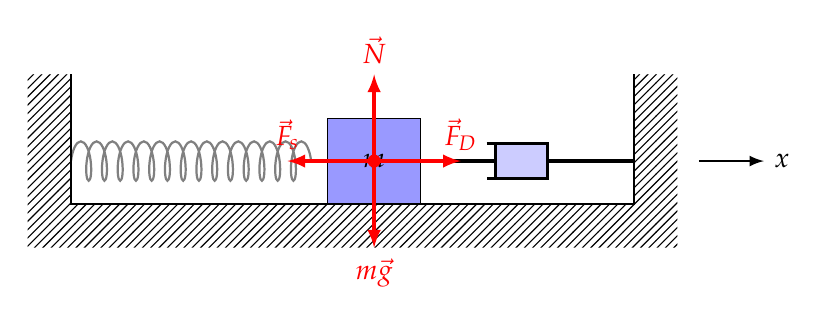
\begin{tikzpicture}[scale=1.1]
      \node[draw,fill=blue!40!white,inner sep=4.5mm] (a) at (3.5,1) {$m$};
      \draw[thick,draw=black!50,
        decoration={aspect=0.3,segment length=2mm, amplitude=2.5mm, coil},
        decorate] (0,1)--(2.95,1);
      \fill[pattern=north east lines](-.5,2)--(-.5,0)--(7,0)--(7,2)--(6.5,2)
      --(6.5,.5)--(0,.5)--(0,2)--cycle;
      \draw[thick] (0,2)--(0,.5)--(6.5,.5)--(6.5,2);
      \draw[->,thick](7.25,1)--(8,1) node[right]{$x$};
      \uncover<2->{
        \draw[fill=blue!20!white] (4.9,.8) rectangle(5.5,1.2);
        \begin{scope}[very thick]
          \draw(4.05,1)--(4.9,1);
          \draw(4.9,.8)--(4.9,1.2);
          \draw(4.8,1.2)--(5.5,1.2)--(5.5,.8)--(4.8,.8);
          \draw(5.5,1)--(6.5,1);
        \end{scope}
      }
      \uncover<3->{
        \fill[red] (3.5,1)circle(.075);
        \begin{scope}[very thick,->,red]
          \draw(3.5,1)--(3.5,0) node[below]{$m\vec g$};
          \draw(3.5,1)--(3.5,2) node[above]{$\vec N$};
          \draw(3.5,1)--(2.5,1) node[above]{$\vec F_s$};
          \draw(3.5,1)--(4.5,1) node[above]{$\vec F_D$};
        \end{scope}
      }
    \end{tikzpicture}
  \end{center}
  \uncover<4->{
    \vspace{-.1in}The damping force is typically related to velocity, in the
    opposite direction:

    \eq{-.12in}{
      \vec F_D=-b(\vec v)^n
    }

    \vspace{-.12in}where $b$ is a positive constant. In the simplest case is to
    use $n=1$ to represent viscous effects. (For kinetic friction, $n=0$; for
    aerodynamic drag, $n=2$.)
  }
\end{frame}



\begin{frame}{Damped Oscillator}
  The 2nd-order ODE is obtained by applying second law of motion, this time
  with the additional term from the damping force:

  \eq{-.1in}{
    \sum F=F_s+{\color{red}F_D}=ma\quad\rightarrow\quad
    -kx{\color{red}-b\dot x}=m\ddot x
  }

  Arranging into standard form:
  
  \eq{-.1in}{
    \ddot x+\frac bm\dot x+\frac kmx=0
  }

  The solution to this ODE is still relatively straightforward (but not as
  easy).
\end{frame}



\begin{frame}{Damped Oscillator}
  The solution to this ODE\footnote{This is still a standard problem in
    calculus.} has both an {\color{red}exponential decay term} and a
  {\color{blue}sinusoidal term}:

  \eq{-.1in}{
    x(t)=A_0{\color{red}e^{-\frac b{2m}t}}{\color{blue}\cos(\omega t+\phi)}
  }

  \vspace{-.1in}where $A_0$ is the initial amplitude of the damped oscillator,
  and the ``natural frequency'' for the damped oscillator is given by:

  \eq{-.1in}{
    \omega=\sqrt{\omega_0^2-\left(\frac b{2m}\right)^2}
  }
  
  Note that $\omega<\omega_0$ (natural frequency decreases) because of the
  damping factor $b$.
  \vspace{.2in}
\end{frame}



\begin{frame}{Critical Damping}
  \textbf{Critical damping} occurs when the natural frequency $\omega$ is zero,
  i.e.:
  
  \eq{-.1in}{
    \sqrt{\omega_0^2-\left(\frac b{2m}\right)^2}=0
  }

  which corresponds to a damping constant:

  \eq{-.1in}{
    b_c=2m\omega_0=2\sqrt{km}
  }
  \begin{itemize}
  \item A critically damped system returns to its equilibrium
    position in the shortest time with \emph{no} oscillation
  \item When $b>b_c$, the system is \textbf{over-damped}
  \item Critical or near-critical damping is desired in many engineering designs
    (e.g.\ shock absorbers on car suspensions)
  \end{itemize}
\end{frame}



\begin{frame}{Comparing Damped System}
  \centering
  \pic{.5}{oscda8}
  
  The motion of the damped oscillator is not strictly periodic.
\end{frame}



\begin{frame}{Energy in a Damped System}
  The non-conservative damping force dissipates energy from the oscillator at
  a rate of:

  \eq{-.1in}{
    P=\diff Et=\vec F_D\cdot\vec v=-bv^2
  }

  As velocity relate to energy by: $(v_{av})^2=E/m$, power dissipation is a
  first-order linear ODE:

  \eq{-.1in}{
    \diff Et=-\frac bmE
  }

  The solution to the ODE shows the total amount of energy decreases
  exponentially with time:

  \eq{-.1in}{
    E(t)=E_0e^{-\frac bmt} %=E_0e^{-\frac{t}{\tau}}
    }
\end{frame}



\section{Driven Oscillation}

\begin{frame}{Forced Harmonic Motion}
  To keep a damped system going, energy must be added into the system. Assuming
  that the system is subjected to an external force ($F_E$) that is harmonic
  with time, with a driving frequency $\omega_E$:

  \eq{-.1in}{
    F_E=F\cos(\omega_Et)
  }
  
  \vspace{-.2in}
  \begin{center}
    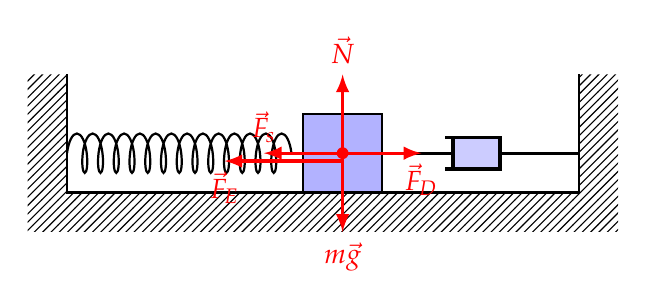
\begin{tikzpicture}
      \draw[thick,fill=blue!30](3,.5) rectangle(4,1.5);
      \draw[thick,
        decoration={aspect=0.3,segment length=2mm, amplitude=2.5mm, coil},
        decorate] (0,1)--(3,1);
      \fill[pattern=north east lines](-.5,2)--(-.5,0)--(7,0)--(7,2)--(6.5,2)
      --(6.5,.5)--(0,.5)--(0,2)--cycle;
      \draw[thick] (0,2)--(0,.5)--(6.5,.5)--(6.5,2);
      \draw[fill=blue!20!white] (4.9,.8) rectangle(5.5,1.2);
      \begin{scope}[very thick]
        \draw(4.05,1)--(4.9,1);
        \draw(4.9,.8)--(4.9,1.2);
        \draw(4.8,1.2)--(5.5,1.2)--(5.5,.8)--(4.8,.8);
        \draw(5.5,1)--(6.5,1);
      \end{scope}
      \fill[red] (3.5,1)circle(.075);
      \begin{scope}[very thick,->,red]
        \draw(3.5,1)--(3.5,0) node[below]{$m\vec g$};
        \draw(3.5,1)--(3.5,2) node[above]{$\vec N$};
        \draw(3.5,1)--(2.5,1) node[above]{$\vec F_s$};
        \draw(3.5,.9)--(2,.9) node[below]{$\vec F_E$};
        \draw(3.5,1)--(4.5,1) node[below]{$\vec F_D$};
      \end{scope}
    \end{tikzpicture}
  \end{center}
  In general, the driving frequency $\omega_E$ does not have to be related to
  the natural frequency $\omega_0$ or damped frequency $\omega$.
\end{frame}



\begin{frame}{Forced Harmonic Motion}
  Again, the second-order ordinary differential equation is obtained by
  applying the second law of motion:
  
  \eq{-.1in}{
    \sum F=-kx-bv+F\cos(\omega_Et)=ma
  }

  Rearranging the terms gives a similar ODE to the damped case, but with the
  \textcolor{green!80!black}{additional external force term} on the right-hand
  side:

  \eq{-.1in}{
    m\ddot x+b\dot x+kx=
    \textcolor{green!80!black}{F\cos(\omega_Et)}
  }
\end{frame}



\begin{frame}{Forced Harmonic Motion}
  \eq{0in}{
    m\ddot x+b\dot x+kx=F\cos(\omega_E t)
  }
  
  The solution to this ODE has two components:
  \begin{itemize}
  \item A \textbf{transient solution} that is identical to that of the damped
    oscillator
    \begin{itemize}
    \item Obtained by setting the external force term to zero
    \item Depends on the initial condition
    \item Solution becomes negligible over time because of exponential-decay
    \end{itemize}
  \item A \textbf{steady-state solution} which does not depend on the initial
    condition
  \end{itemize}
\end{frame}



\begin{frame}{Forced Harmonic Motion}
  Solving for the steady-state solution will be left as a difficult calculus
  exercise\footnote{usually taught in 2nd-year university level ODE course},
  but it can be shown that the solution is a harmonic motion at the driving
  frequency $\omega_E$ of the external force:

  \eq{-.1in}{
    \boxed{x(t)=A\cos(\omega_E t-\phi)}
  }
  
  where the amplitude of the oscillation $A$ and phase shift $\phi$ are given
  by:

  \eq{-.1in}{
    A=\frac F{\sqrt{m^2(\omega_0^2-\omega_E^2)^2+b^2\omega_E^2}}
    \quad\;\;
    \tan\phi=\frac{b\omega_E}{m(\omega_0^2-\omega_E^2)}
  }
  \vspace{.3in}
\end{frame}



\begin{frame}{Resonance}
  \textbf{Resonance} is caused by in-phase excitation at natural frequency.
  This means that:
  \begin{itemize}
  \item The frequency of the driving force is \emph{approximately} the natural
    frequency of the damped oscillator:

    \eq{-.1in}{
      \omega_E=\sqrt{\omega_0-\frac b{2m}}
      \quad\text{where}\quad\omega_0=\sqrt{\frac km}
    }

    For a lightly damped system, this means that $\omega_E\approx\omega$
    
  \item The driving force follows the motion of the oscillator.
  \end{itemize}
\end{frame}



\begin{frame}{Resonance}
  \eq{-.1in}{
    A=\frac F{\sqrt{m^2(\omega_0^2-\omega_E^2)^2+b^2\omega_E^2}}
  }
  
  Maximum $A$ occurs when the denominator is the smallest, which can be related
  to the external frequency by setting the derivative with respect to
  $\omega_E$ to 0:

  \eq{-.1in}{
    \diff{}{\omega_E}\left[m^2(\omega_0^2-\omega_E^2)^2+b^2\omega_E^2\right]=0
  }

  It is a simple exercise
  %\footnote{$b$, $m$ and $\omega_o$ are all constants anyway!}
  to see that the minimum value occurs at the natural frequency of
  the damped oscillator.

  \eq{-.1in}{
    \omega_E=\sqrt{\omega_0-\frac b{2m}}
  }
%  The maximum amplitude is:
%  
%  \eq{-.2in}{
%    A_\text{max}=\frac F{b\omega_E}
%  }
\end{frame}



\begin{frame}{Resonance}
  \begin{columns}
    \column{.55\textwidth}
    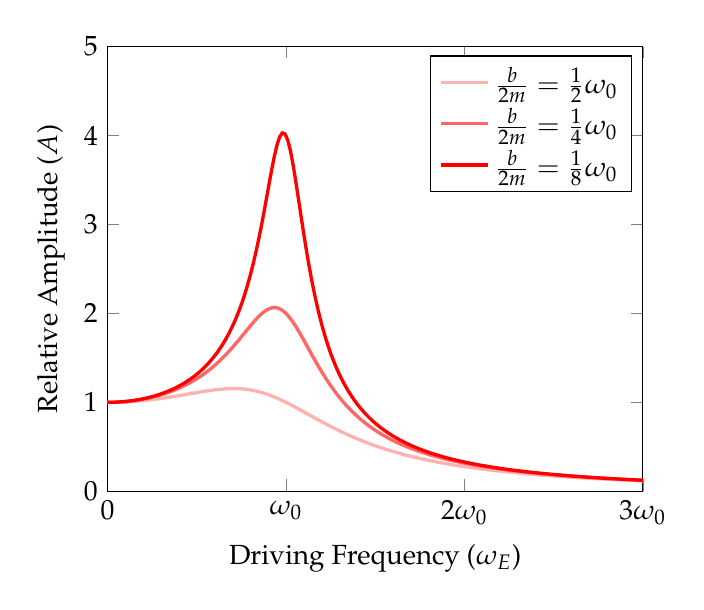
\begin{tikzpicture}
      \begin{axis}[
          width=3.3in,
          xmin=0,xmax=3, xlabel=Driving Frequency ($\omega_E$),
          xtick={0,1,2,3}, xticklabels={0,$\omega_0$,$2\omega_0$,$3\omega_0$},
          ymin=0,ymax=5, ylabel=Relative Amplitude ($A$),
        ]
        \addplot[
          color=red!30,
          samples=300,
          domain=0:3,
          very thick]{1/sqrt((1-x^2)^2+x^2)};
        \addlegendentry{$\frac b{2m}=\frac12\omega_0$};
        \addplot[
          color=red!60,
          samples=200,
          domain=0:3,
          very thick]{1/sqrt((1-x^2)^2+x^2/4)};
        \addlegendentry{$\frac b{2m}=\frac14\omega_0$};
        \addplot[
          color=red,
          samples=200,
          domain=0:3,
          very thick]{1/sqrt((1-x^2)^2+x^2/16)};
        \addlegendentry{$\frac b{2m}=\frac18\omega_0$};
      \end{axis}
    \end{tikzpicture}

    \column{.45\textwidth}
    Plotting amplitude $A$ as a function of driving frequency $\omega$ shows
    that:
    \begin{itemize}
    \item For a lightly damped system (i.e.\ small $b$), resonance response is
      highest when $\omega_E\approx\omega\approx\omega_0$
    \item The smaller the damping constant $b$, the higher and narrower the
      peak is
    \end{itemize}
  \end{columns}
\end{frame}



\begin{frame}{Resonance}
  \eq{0in}{
    \boxed{\tan\phi=\frac{b\omega_E}{m(\omega_0^2-\omega_E^2)}}
  }

  When $\omega_E=\omega_0$ is substituted into the phase shift expression, the
  right-hand side becomes undefined. From this, we obtain a phase shift of
  $\phi=\pi/2$. Taking derivative of $x(t)$ for velocity $v(t)$, and
  substituting $\phi=\pi/2$:
  
  \eq{-.1in}{
    v(t)=\dot x
    =-A\omega_E\sin(\omega_E t-\frac{\pi}2)
    =A\omega_E\cos(\omega_E t)
  }
\end{frame}



\begin{frame}{Resonance}
  At resonance, the object is always moving in the same direction as the
  driving force:

  \vspace{-.3in}{\large
    \begin{align*}
      v(t)&=A\omega_E\cos(\omega_E t)\\
      F_E(t)&=F\cos(\omega_E t)
    \end{align*}
  }

  \vspace{-.2in}This also makes sense from a work-energy perspective, because
  now the external force is doing positive work to the system.
\end{frame}
\end{document}
